\documentclass[12pt]{article}
\usepackage{verbatim}
\usepackage[dvips]{epsfig}
\usepackage{color}
\usepackage{url}
\usepackage[colorlinks=true]{hyperref}

\begin{document}

\section*{GENESIS: Documentation}

{\bf Related Documentation:}
% start: userdocs-tag-replace-items related-build-debian
% end: userdocs-tag-replace-items related-build-debian

\section*{Building Debian Packages for GENESIS Components}

This guide describes how to build a \href{http://www.debian.org/doc/manuals/apt-howto/index.en.html#contents}{Debian package} for a \href{../reserved-words/reserved-words.tex}{GENESIS component}. It uses installer scripts included with the \href{../developer-package/developer-package.tex}{\it DeveloperPackage}.

\subsection*{Dependencies}

Before you can build a Debian package you need to have the following packages installed on the machine.
\begin{itemize}
   \item{\it dh-make}
   \item{\it dpkg-dev}
   \item{\it dpkg}
\end{itemize}

If you are using the \href{http://www.ubuntu.com/}{Ubuntu operating system}, all three are available from \href{http://www.debian.org/doc/manuals/apt-howto/}{\it apt-get} and \href{http://www.nongnu.org/synaptic/}{Synaptic Package Manager}.


\subsection*{Utilities}
\begin{itemize}
\item {\it nspkg-deb}: Checks for all files needed to build a Debian package and performs the build.
\end{itemize}
\subsection*{Configuration Files}

To build a Debian package you need the following files specific to the package you are building:
\begin{itemize}
\item {\it control}: Has information like the package name, dependencies, and package information.
\item {\it rules}: Contains build instructions.
\item {\it changelog}: A log file that shows the date, author, and context of the last change made to the package.
\item {\it copyright}: Contains the author and distribution license. 
\end{itemize}

A detailed explanation of each file follows.

\subsubsection*{control file}

The control file is a series of fields which correspond to information about the package you are building.
\begin{itemize}
\item {\bf Source:} The source package name ({\color{red}mandatory}).
\item {\bf Section:} Classification for the package.
\item {\bf Priority:} Importance of installation to the user, all of GENESIS can be labeled ``{\tt optional}''.
\item {\bf Maintainer:} The name and address of the packager ({\color{red}mandatory}).
\item {\bf Build-Depends:} This holds dependencies that are checked when performing a build.
\item {\bf Homepage:} The URL of the website for the package.
\item {\bf Package:} The name of the binary package ({\color{red}mandatory}).
\item {\bf Architecture:} Which architecture the package is for, all GENESIS packages are labeled `{\tt any}'.
\item {\bf Depends:} This holds dependencies that are checked during configuration.
\item {\bf Suggests:} Recommended software.
\item {\bf Description:} A textual description of the package and its uses. 
\end{itemize}
Example taken from the {\it DeveloperPackage}:
\begin{verbatim}
   Source: Developer
   Section: Science 
   Priority: optional
   Maintainer: Hugo Cornelis [hugo.cornelis@gmail.com]
   Build-Depends: python2.5(>=2.5),libc6(>=2.3.6),libgcc1 (>=4.1.1)
   Homepage: http://neurospaces.sourceforge.net/
   
   Package: neurospaces-developer-package
   Architecture: any
   Depends: python2.5(>=2.5),libc6(>=2.3.6),libgcc1 (>=4.1.1)
   Suggests: gnuplot
   Description: The Neurospaces developer package contains essential tools for Neurospaces development.
\end{verbatim}

\subsubsection*{rules file}

This is a file with {\it make} instructions that are called when {\it dpkg-buildpackage} is invoked. It contains a rule for each source in the package.

The rules file used in the GENESIS packages is based on an example from Joey Hess from the Debian forums.

\subsubsection*{changelog}

This is a log of the changes made to the package by the maintainer. This file has a particular format that must be followed, otherwise the package build will fail, halting the packaging process.

Example from the {\it DeveloperPackage}.
\begin{verbatim}
   Developer (alpha.1) dapper; urgency=low
      * First release packaged for ubuntu
      -- Hugo Cornelis <hugo.cornelis@gmail.com>  Sat, 8 Aug 2009 14:45:16 +0000
\end{verbatim}

The date in particular must follow the shown format of:

    {\bf Day of the week, Day Month Year Time} 

as shown in the above example.

\subsubsection*{copyright file}

File contains copyright info. All components of the GENESIS project are licensed under GPL.

\subsubsection*{Important Note about config files}

The package identifier must be identical in the following locations:
\begin{itemize}
   \item The first line in the changelog file.
   \item Source and Package tags in the control file.
   \item The {\tt make install DESTDIR=\$(CURDIR)/debian/<packagename>} line in the install target of the rules file. Where {\tt <packagename>} is the name of the package to be built. 
\end{itemize}
Otherwise the build will fail. A log of a Debian build can be found in {\it build\_debian.log} file in the top level directory.

\subsubsection*{Checking your package}

Once you have your {\bf .deb} file in the top level source directory there are a couple ways you can go about verifying its contents. 

If you wish to view the package contents via a gui interface, there is {\it deb-gview} which is available via {\it apt-get} and the synaptic package manager. Opening  the resulting package in {\it deb-gview} you get a nice listing of all the files in the package as well as the package information:


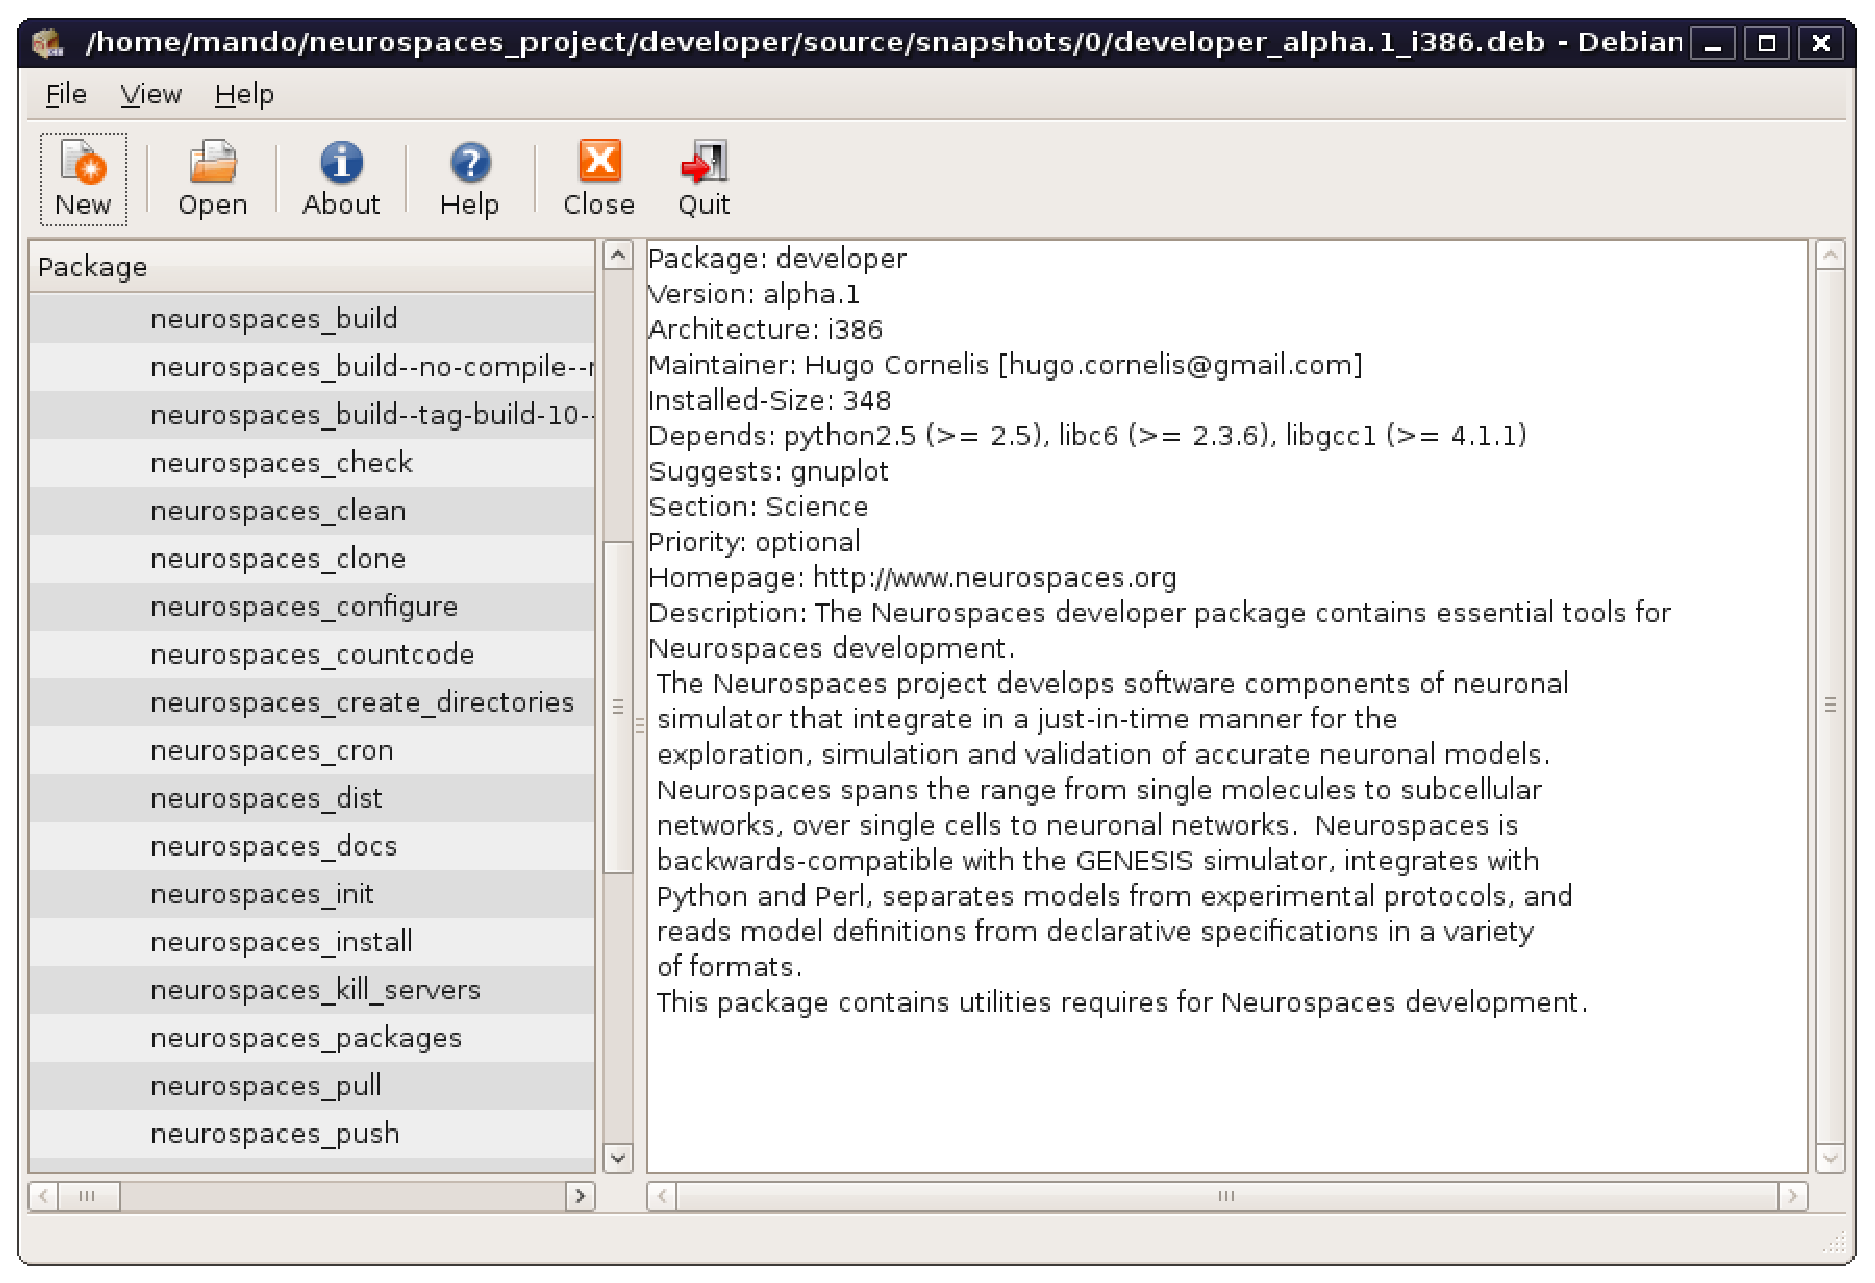
\includegraphics[scale=0.4]{figures/deb-gview.eps}

You can also verify package contents via the command line using {\it lintian}, which is also available via apt-get and synaptic package manager. In addition to verifying the package contents, {\it lintian} will point out errors in the package build data. 



\end{document}
